%%%%%%%%%%%%%%%%%%%%%%%%%%%%%%%%%%%%%%%%%%%%%%%%%%%%%%%%%%%%%%%%%%%%%%%%%%%%%%%%%
% This is an example CV created using maincv.cls (v1.0, 21 April 2021) written by
% Victor Skurikhin (vskurikhin@gmail.com).
%
%% It may be distributed and/or modified under the
%% conditions of the LaTeX Project Public License, either version 1.3
%% of this license or (at your option) any later version.
%% The latest version of this license is in
%%    http://www.latex-project.org/lppl.txt
%% and version 1.3 or later is part of all distributions of LaTeX
%% version 2003/12/01 or later.
%%%%%%%%%%%%%%%%%%%%%%%%%%%%%%%%%%%%%%%%%%%%%%%%%%%%%%%%%%%%%%%%%%%%%%%%%%%%%%%%%

\documentclass[10pt,a4paper,ragged2e]{maincv}

%% V-N-Skurikhin uses the fontawesome and academicon fonts
%% and packages.
%% See texdoc.net/pkg/fontawecome and http://texdoc.net/pkg/academicons for full list of symbols.
%% You MUST compile with XeLaTeX or LuaLaTeX if you want to use academicons.

\usepackage[english,russian]{babel}

\PassOptionsToPackage{dvips}{graphics} 
\graphicspath{{images/}}

% Change the page layout if you need to
\geometry{left=2cm,right=9.5cm,marginparwidth=7.75cm,marginparsep=0.5cm,top=1.25cm,bottom=1.25cm}

% Change the font if you want to, depending on whether
% you're using pdflatex or xelatex/lualatex
\ifxetexorluatex
  % If using xelatex or lualatex:
  \setmainfont{Carlito}
\else
  % If using pdflatex:
  \usepackage[utf8]{inputenc}
  \usepackage[T1]{fontenc}
  \usepackage[default]{lato}
  \usepackage{blindtext}
\fi

% Change the colours if you want to
\definecolor{VividPurple}{HTML}{000000}
\definecolor{SlateGrey}{HTML}{2E2E2E}
\definecolor{LightGrey}{HTML}{2E2E2E}
\colorlet{heading}{VividPurple}
\colorlet{accent}{VividPurple}
\colorlet{emphasis}{SlateGrey}
\colorlet{body}{LightGrey}

% Change the bullets for itemize and rating marker
% for \cvskill if you want to
\renewcommand{\itemmarker}{{\small\textbullet}}
\renewcommand{\ratingmarker}{\faCircle}

%% sample.bib contains your publications
\addbibresource{sample.bib}

\begin{document}

\begin{tabular}[l]{lll}
\ & \ & \multirow{2}{6cm}{\includegraphics[width=4.25cm]{V-N-Skurikhin.eps}} \\[4mm]
{\fontsize{25}{35}\selectfont \textbf{Виктор Николаевич Скурихин}} & \ & \\[4mm]
\fontsize{15}{25}\selectfont \textbf{Руководитель направления разработки} & \ & \\[3mm]
\email{vskurikhin@gmail.com} & \ & \\[2mm]
\phone{+79015499556} & \ & \\[2mm]
\location{Московская область, Россия} & \ & \\[2mm]
\github{https://github.com/vskurikhin/resume} & \ & \\[2mm]
\homepage{https://svn.su} & \ &
\end{tabular}

%% Depending on your tastes, you may want to make fonts of itemize environments slightly smaller
\AtBeginEnvironment{itemize}{\small}

%% Provide the file name containing the sidebar contents as an optional parameter to \cvsection.
%% You can always just use \marginpar{...} if you do
%% not need to align the top of the contents to any
%% \cvsection title in the "main" bar.
\cvsection[page1sidebar]{Опыт}
\justifying
\hyphenation{thatshouldnot}

\cveventv{Руководитель направления разработки}{Сбербанк (Крупнейший универсальный банк России)}
{Июнь 2020 -- по настоящее время}{Москва, РФ}{0.608}
\begin{itemize}
\item
{Формирование и развитие команды, постановка задач разработчикам и контроль их выполнения.
Подбор специалистов и проведение технических собеседований.
}
\item
{{\hyphenation{thatshouldnot}Разработка и внедрение кода. Знание процесса разработки,} \begin{sloppypar}умение его организовывать и оптимизировать.\end{sloppypar}
Умение писать хорошо структурированный, документированный, понятный другим разработчикам код, используя современные стандарты и технологии.
}
\smallskip
\item {
\sloppy{Микросервисный продукт часть мобильного приложения \begin{sloppypar}СберИнвестиции.\end{sloppypar}}}
\end{itemize}

\divider

\cveventv{Главный инженер разработки}{Газпромбанк (Один из крупнейших банков России)}
{Июль 2019 -- Июнь 2020}{Москва, Россия}{0.461}
\begin{itemize} 
\item {\sloppy{Разрабатывал высоконагруженную автоматизированную систему обработки кредитных заявок, участвующей
в процессе корпоративного кредитования.}}
\smallskip
\item
{Участвовал в решении задач на всех этапах от оценки входящих требований бизнеса до внедрения.}
\end{itemize}

\divider

\cveventv{Главный эксперт}{UniCredit Bank (Российский коммерческий банк)}
{Октябрь 2017 -- Июнь 2019}{Москва, Россия}{0.51}
\begin{itemize}
\item {Разрабатывал промышленные системы на основе SOAP. Участвовал в проектах с учётом полного технологического цикла.
 Поддерживал Core-banking кластеры.}
\smallskip
\item {Участвовал в инициативной группе по внедрению CI/CD практик. Разворачивал пилотный проект на OpenShift.}
\end{itemize}

\divider

\cveventv{Главный специалист}{Газпром информ (Дочерняя компания ПАО «Газпром»)}
{Август 2011 -- Cентябрь 2017}{Москва, Россия}{0.537}
\begin{itemize}
\item Сопровождал cистему Документооборота ПАО «Газпром».
\end{itemize}

\divider

\cveventv{Старший Системный Администратор}{Райффайзенбанк (Российский коммерческий банк)}
{Август 2007 -- Август 2011}{Москва, Россия}{0.496}
\begin{itemize}
\item Поддерживал промышленные операционные системы.
\end{itemize}

% \divider
\clearpage

\newgeometry{left=2cm,right=10.5cm,marginparwidth=8.3cm,marginparsep=0.75cm,top=1.25cm,bottom=1.25cm}

\begin{fullwidth}

\cvsection{Повышение квалификации}

\cvevent{Профессиональная переподготовка в сфере Информационные технологии.}
{ФГБУ ВО и Науки, Санкт-Петербургский Национальный Исследовательский Академический \mbox{Университет} Российской Академии Наук}
{2015 -- 2016}{}

\end{fullwidth}

\cvsection[page2sidebar]{Экзамены}

\cvevent{IBM Certified Systems Expert}{High Availability for AIX Administration - v2}{2013}{IBM/Prometric}
\cvevent{IBM Certified Systems Expert}{Virtualization Technical Support for AIX and Linux}{2012}{IBM/Prometric}
\cvevent{IBM Certified System Administrator AIX 7}{Power Systems with AIX v3}{2012}{IBM/Prometric}
\cvevent{Oracle Solaris 10 System Administrator}{Certified Professional Exam}{2011}{Pearson VUE}

\begin{fullwidth}

\cvsection{Курсы}

\cvevent{}{Highload Architect, Otus - 2021}{}{}
\cvevent{}{Разработчик на Spring Framework, Otus - 2019}{}{}
\cvevent{}{Разработчик Java Enterprise, Otus - 2018}{}{}
\cvevent{}{Разработчик Java, Otus - 2018}{}{}
\cvevent{}{HPE Accelerated SAN Essentials UC434S - 2017}{}{}
\cvevent{}{Функциональное программирование на языке Haskell (часть 2), Computer Science Center - Stepik - 2017}{}{}
\cvevent{}{Функциональное программирование на языке Haskell, Computer Science Center - Stepik - 2016}{}{}
\cvevent{}{Многопоточное программирование на С/С++ - Mail.Ru - Stepik - 2016}{}{}
\cvevent{}{An Introduction to Interactive Programming in Python (Part 2), Coursera - RICE - 2015}{}{}
\cvevent{}{An Introduction to Interactive Programming in Python (Part 1), Coursera - RICE - 2015}{}{}

\end{fullwidth}

\clearpage

\nocite{*}

\end{document}
